\documentclass{article}
% Examen Statistiek 6OB (75 minuten) - LaTeX-bron, met pandoc naar Word
\newcommand{\lijn}{\par LIJN\par}
\newcommand{\gat}[1]{\textsc{#1}}
\newcommand{\pagina}{\par PAGEBREAK\par}
\newcommand{\breedtes}[1]{\par BREEDTE:#1\par}

\begin{document}

\begin{banner}
EXAMEN WISKUNDE \quad·\quad 6 OPVOEDING EN BEGELEIDING
\end{banner}

\begin{titel}
Examen Statistiek
\end{titel}

\begin{ondertitel}
Basisbegrippen in de statistiek · Kengetallen
\end{ondertitel}

\textbf{Tijdsduur:} 75 minuten – \textbf{Totaal:} \_\_\_ / 50

\textbf{Naam:} \_\_\_\_\_\_\_\_\_\_\_\_\_\_\_\_\_\_\_\_\_\_\_\_\_\_\_\_\_\_ \quad \textbf{Klas:} \_\_\_\_\_\_\_\_\_\_\_\_\_ \quad \textbf{Datum:} \_\_\_\_\_\_\_\_\_\_\_\_\_

\begin{letop}
\textbf{1.} Werk nauwkeurig en ordelijk.

\textbf{2.} Gebruik een kladblad. Schrijf je naam op het kladblad.

\textbf{3.} Lees elke vraag aandachtig.

\textbf{4.} Noteer je berekeningen en redeneringen. Een antwoord zonder werkwijze krijgt niet alle punten.

\textbf{5.} Je mag je rekentoestel en GeoGebra of Excel gebruiken.

\textbf{6.} Rond af op 2 decimalen, tenzij anders vermeld.
\end{letop}

\textbf{Veel succes!}

% ---------------------------------------------------------------- Vraag 1
\breedtes{82/18}
\begin{tabular}{lc}
\hline
Vraag 1 · Stappen van een statistisch onderzoek & \_\_\_ / 4 \\
\hline
\end{tabular}

Een kinderopvang onderzoekt waarom kinderen ’s middags moeilijk in slaap vallen. Vier uitspraken uit het onderzoek:

\textbf{(1)} De opvang merkt dat veel kinderen na het middageten moeilijk in slaap vallen.

\textbf{(2)} Hoeveel minuten hebben de kinderen nodig om in te slapen na het middageten?

\textbf{(3)} De opvang veronderstelt dat de meeste kinderen langer dan 20 minuten nodig hebben.

\textbf{(4)} Uit de metingen blijkt dat de kinderen gemiddeld 24 minuten nodig hebben.

\textbf{a)} Welke stap van het onderzoek is elke uitspraak: probleemstelling, onderzoeksvraag, hypothese of conclusie? (1) \_\_\_\_\_\_\_\_ (2) \_\_\_\_\_\_\_\_ (3) \_\_\_\_\_\_\_\_ (4) \_\_\_\_\_\_\_\_ \hfill \textbf{\_\_\_ / 2} 

\textbf{b)} Zet deze vier stappen in de juiste volgorde: \textbf{A} conclusies trekken – \textbf{B} data verzamelen – \textbf{C} reflecteren en communiceren – \textbf{D} data analyseren en samenvatten. Volgorde: \_\_ – \_\_ – \_\_ – \_\_ \hfill \textbf{\_\_\_ / 2} 

\begin{oplossing}
\textbf{Oplossing 1} \quad a) (1) probleemstelling, (2) onderzoeksvraag, (3) hypothese, (4) conclusie (½ punt per juiste benaming). b) B – D – A – C (2 p; 1 p als één stap verkeerd staat; 0 p bij meer fouten).
\end{oplossing}

% ---------------------------------------------------------------- Vraag 2
\breedtes{82/18}
\begin{tabular}{lc}
\hline
Vraag 2 · Variabelen, data en dataset & \_\_\_ / 4 \\
\hline
\end{tabular}

Een jeugdhuis bevraagt zijn bezoekers. Noteer bij elke vraag de onderzochte variabele, of die kwalitatief of kwantitatief is en welk soort data erbij hoort (numeriek, categorisch geordend of categorisch niet-geordend).

\breedtes{42/20/20/18}
\begin{tabular}{llll}
\hline
Enquêtevraag & Variabele & Kwalitatief of kwantitatief? & Soort data \\
\hline
a) Hoeveel keer per maand kom je naar het jeugdhuis? & & & \\
b) Hoe tevreden ben je over het aanbod? (zeer ontevreden – ontevreden – neutraal – tevreden – zeer tevreden) & & & \\
c) In welke gemeente woon je? & & & \\
\hline
\end{tabular}

\textbf{(1 punt per rij)}

\textbf{d)} Hoe noemt men de verzameling van alle antwoorden uit het onderzoek? \hfill \textbf{\_\_\_ / 1} \lijn 

\begin{oplossing}
\textbf{Oplossing 2} \quad a) aantal bezoeken per maand; kwantitatief; numeriek (1). b) tevredenheid over het aanbod; kwalitatief; categorisch geordend (1). c) gemeente van de bezoeker; kwalitatief; categorisch niet-geordend (1). Per rij 1 punt als variabele, soort variabele én soort data juist zijn; ½ punt als één van de drie ontbreekt of fout is. d) de dataset (1).
\end{oplossing}

% ---------------------------------------------------------------- Vraag 3
\breedtes{82/18}
\begin{tabular}{lc}
\hline
Vraag 3 · Steekproef en populatie & \_\_\_ / 5 \\
\hline
\end{tabular}

Een woonzorgcentrum telt 240 bewoners. Om te weten hoeveel uur per dag bewoners aan activiteiten deelnemen, worden 40 geloote bewoners bevraagd. Het gemiddelde is 2,6 uur en de standaardafwijking is 0,8 uur.

\textbf{a)} Noteer de populatie, de steekproef, $N$ en $n$. \hfill \textbf{\_\_\_ / 1} \lijn 

\textbf{b)} Noteer de twee getallen uit de tekst met de juiste symbolen en zeg welke populatieparameters ze schatten. \hfill \textbf{\_\_\_ / 1} \lijn 

\textbf{c)} Een ander team bevraagt 40 andere geloote bewoners en vindt een gemiddelde van 2,9 uur. Verklaar waarom dit niet verwonderlijk is. \hfill \textbf{\_\_\_ / 1} \lijn 

\textbf{d)} Noem een reden waarom men een steekproef onderzoekt in plaats van alle 240 bewoners, en een reden waarom dat in andere onderzoeken nodig kan zijn. \hfill \textbf{\_\_\_ / 1} \lijn \lijn 

\textbf{e)} Welke vorm van statistiek is elke uitspraak: verzamelende, beschrijvende of verklarende? (i) De vragenlijst wordt aan 40 bewoners voorgelegd. (ii) De antwoorden worden samengevat in een tabel en een gemiddelde. (iii) Men besluit: ‘Bewoners van Vlaamse woonzorgcentra nemen gemiddeld 2,6 uur per dag deel aan activiteiten.’ (i) \_\_\_\_\_\_\_\_ (ii) \_\_\_\_\_\_\_\_ (iii) \_\_\_\_\_\_\_\_ \hfill \textbf{\_\_\_ / 1} 

\begin{oplossing}
\textbf{Oplossing 3} \quad a) Populatie: alle 240 bewoners ($N=240$); steekproef: de 40 geloote bewoners ($n=40$) (1). b) $\overline{x}=2{,}6$ uur schat $\mu$ en $s=0{,}8$ uur schat $\sigma$ (1). c) Steekproefvariabiliteit: een andere steekproef bevat andere bewoners en geeft door toeval een ander resultaat (1). d) Bijvoorbeeld: te duur of te veel tijd om alle bewoners te bevragen; andere redenen: ethische redenen, of het onderzoek vernietigt de populatie (bv. testen tot een product breekt) (1: twee redenen). e) (i) verzamelende, (ii) beschrijvende, (iii) verklarende (1 p als alle drie juist; ½ p bij twee juist).
\end{oplossing}

% ---------------------------------------------------------------- Vraag 4
\breedtes{82/18}
\begin{tabular}{lc}
\hline
Vraag 4 · Steekproefontwerp & \_\_\_ / 6 \\
\hline
\end{tabular}

Een kinderopvang wil weten hoe de 240 ouders de nieuwe openingsuren vinden. Er wordt een vragenlijst aan de ingang gehangen. Er worden 36 vragenlijsten ingevuld.

\textbf{a)} Bereken het responspercentage. \hfill \textbf{\_\_\_ / 1} \lijn 

\textbf{b)} Welke vorm van vertekening en welk probleem bedreigen hier de representativiteit? \hfill \textbf{\_\_\_ / 1} \lijn 

\textbf{c)} Noem de drie criteria waaraan een representatieve steekproef moet voldoen. \hfill \textbf{\_\_\_ / 1} \lijn \lijn 

\textbf{d)} Wat is een enkelvoudig aselecte steekproef? Beschrijf hoe de opvang er een van 60 ouders kan trekken. \hfill \textbf{\_\_\_ / 2} \lijn \lijn \lijn 

\textbf{e)} Welke vorm van vertekening is het? (i) Een leerling bevraagt enkel mensen die het lokale winkelcentrum verlaten. (ii) Een zender vraagt kijkers via sms te stemmen. (i) \_\_\_\_\_\_\_\_\_\_\_\_\_\_ (ii) \_\_\_\_\_\_\_\_\_\_\_\_\_\_ \hfill \textbf{\_\_\_ / 1} 

\begin{oplossing}
\textbf{Oplossing 4} \quad a) $\dfrac{36}{240}\cdot 100\,\%=15\,\%$ (1). b) Vrijwillige respons (enkel wie wil, vult in) en een te grote non-respons (slechts 15 \% antwoordt); eventueel opportunistisch (enkel wie langs de ingang komt) (1, minstens vrijwillige respons én non-respons). c) De steekproefomvang moet voldoende groot zijn; de samenstelling moet overeenkomen met de populatie; de non-respons mag niet te groot zijn (1: alle drie; ½ bij twee). d) Elk element van de populatie heeft dezelfde kans om in de steekproef te komen, door volledig willekeurige trekking (1); elke ouder een nummer 1 – 240 geven en met de computer lukraak 60 verschillende nummers trekken (1). e) (i) opportunistische steekproef, (ii) vrijwillige respons (1 p als beide juist).
\end{oplossing}

% ---------------------------------------------------------------- Vraag 5
\breedtes{82/18}
\begin{tabular}{lc}
\hline
Vraag 5 · Misleidingen en valkuilen & \_\_\_ / 6 \\
\hline
\end{tabular}

Een jeugdbeweging publiceert deze grafiek.

\begin{center}
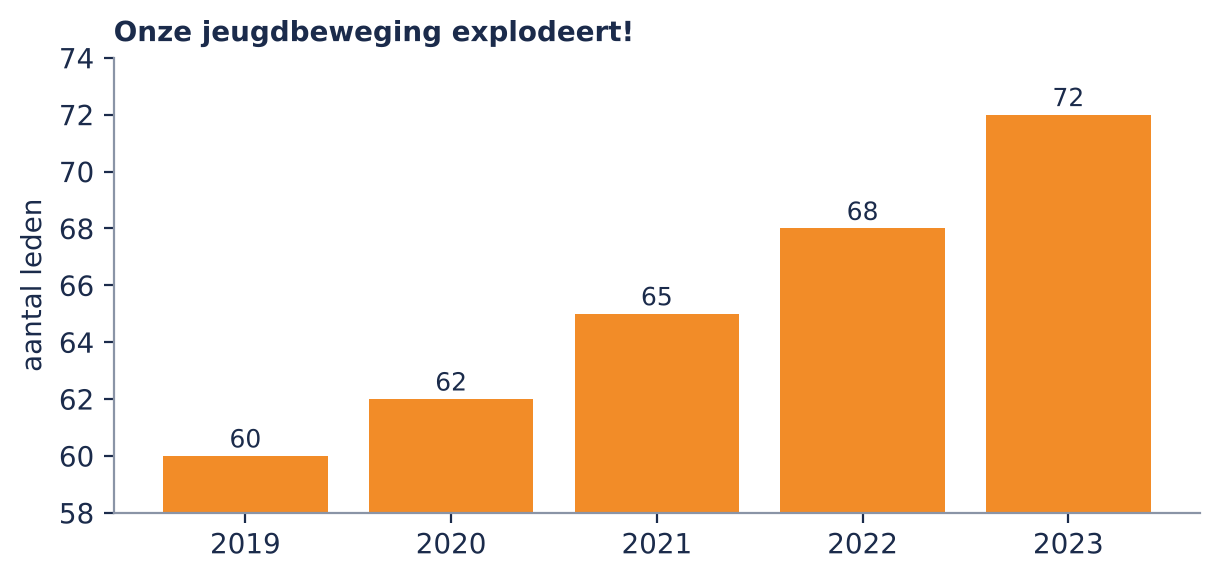
\includegraphics[width=0.7\textwidth]{figuren/exam_staaf.png}
\end{center}

\textbf{a)} Welke misleiding zie je en wat is het misleidende gevolg? \hfill \textbf{\_\_\_ / 1} \lijn 

\textbf{b)} Bereken met ICT met hoeveel procent het aantal leden steeg van 2019 tot en met 2023. \hfill \textbf{\_\_\_ / 1} \lijn 

\textbf{c)} Het aandeel leden dat op kamp gaat, stijgt van 30 \% naar 45 \%. Druk die stijging uit in procentpunt en in procent. \hfill \textbf{\_\_\_ / 1} \lijn 

\textbf{d)} Welke valkuil bij het verzamelen van data zie je? (i) ‘Bent u ook voor een veiliger en gezonder schoolbeleid?’ (ii) ‘9 op 10 ouders vinden onze koekjes gezond’, uit een onderzoek dat de koekjesfabrikant zelf betaalde. \hfill \textbf{\_\_\_ / 2} \lijn \lijn 

\textbf{e)} Waarom kan een 3D-cirkeldiagram misleidend zijn? \hfill \textbf{\_\_\_ / 1} \lijn 

\begin{oplossing}
\textbf{Oplossing 5} \quad a) De verticale as begint bij 58 in plaats van bij 0 (afgeknotte as) (½); daardoor lijkt de groei veel groter dan ze is (½). b) $\dfrac{72-60}{60}=0{,}20=20\,\%$ (1). c) 15 procentpunt (½) en $\dfrac{45-30}{30}=0{,}50=50\,\%$ (½). d) (i) suggestieve vraagstelling (1); (ii) de opdrachtgever heeft belang bij het resultaat (1). e) Wat op de voorgrond staat, lijkt groter dan wat op de achtergrond staat (1).
\end{oplossing}

% ---------------------------------------------------------------- Vraag 6
\breedtes{82/18}
\begin{tabular}{lc}
\hline
Vraag 6 · Samenhang en causaliteit & \_\_\_ / 5 \\
\hline
\end{tabular}

\textbf{a)} Wat is het verschil tussen samenhang (correlatie) en causaliteit? \hfill \textbf{\_\_\_ / 1} \lijn \lijn 

\textbf{b)} Welke redeneerfout zit in elke uitspraak? Kies \textbf{O} (omgekeerde oorzakelijke richting), \textbf{T} (toevallige samenhang) of \textbf{D} (derde variabele) en leg uit.

\textbf{(i)} Kinderen die vaker naar de logopedist gaan, hebben meer spraakproblemen. De logopedist veroorzaakt dus spraakproblemen. \hfill \textbf{\_\_\_ / 1} \lijn \lijn 

\textbf{(ii)} Wijken met meer speeltuinen hebben meer fietsendiefstallen. Noem ook de verborgen variabele. \hfill \textbf{\_\_\_ / 1} \lijn \lijn 

\textbf{(iii)} Het aantal films met een hond in de hoofdrol en het aantal doctoraten in de biologie stijgen over de jaren samen. \hfill \textbf{\_\_\_ / 1} \lijn \lijn 

\textbf{c)} Wat is het verschil tussen observationeel en experimenteel onderzoek? \hfill \textbf{\_\_\_ / 1} \lijn \lijn 

\begin{oplossing}
\textbf{Oplossing 6} \quad a) Samenhang is een statistisch verband tussen twee variabelen (bij kwantitatieve variabelen: correlatie); causaliteit betekent dat de ene variabele de andere rechtstreeks beïnvloedt; samenhang bewijst geen causaliteit (1). b) (i) O: wie spraakproblemen heeft, gaat naar de logopedist (1). (ii) D: bijvoorbeeld het aantal inwoners (of kinderen) in de wijk (1: juiste letter én variabele). (iii) T: geen inhoudelijk verband, de samenhang is toeval (1). c) Observationeel: de onderzoeker grijpt niet in en verzamelt enkel data (enkel samenhang); experimenteel: de onderzoeker grijpt in en bepaalt wie de behandeling krijgt, met randomisatie en een controlegroep (ook causaliteit mogelijk) (1).
\end{oplossing}

% ---------------------------------------------------------------- Vraag 7
\breedtes{82/18}
\begin{tabular}{lc}
\hline
Vraag 7 · Experimenteel onderzoek & \_\_\_ / 4 \\
\hline
\end{tabular}

Een school wil weten of een dagelijkse ‘beweegpauze’ de conditie van leerlingen verbetert. Er worden 200 leerlingen \emph{door loting} verdeeld in een experimentele groep (100, met beweegpauze) en een controlegroep (100, zonder). Na een trimester wordt de conditie gemeten.

\breedtes{28/18/18/18/18}
\begin{tabular}{lcccc}
\hline
 & verbeterd & gelijk & verslechterd & totaal \\
\hline
experimentele groep & 70 & 20 & 10 & \\
controlegroep & 45 & 40 & 15 & \\
totaal & & & & \\
\hline
\end{tabular}

\textbf{a)} Is dit observationeel of experimenteel onderzoek? Waar speelt randomisatie een rol? \hfill \textbf{\_\_\_ / 1} \lijn 

\textbf{b)} Welk percentage van elke groep verbeterde? \hfill \textbf{\_\_\_ / 1} \lijn 

\textbf{c)} Wat is de rol van de controlegroep en waarom verdeelt men de leerlingen door loting? \hfill \textbf{\_\_\_ / 1} \lijn \lijn 

\textbf{d)} Mag je besluiten dat de beweegpauze de conditie verbetert? Verklaar. \hfill \textbf{\_\_\_ / 1} \lijn \lijn 

\begin{oplossing}
\textbf{Oplossing 7} \quad (Totalen: 115 – 60 – 25 – 200.) a) Experimenteel (de onderzoekers grijpen in); randomisatie bij het verdelen van de leerlingen in de twee groepen door loting (1). b) Experimentele groep: $\frac{70}{100}=70{,}0\,\%$; controlegroep: $\frac{45}{100}=45{,}0\,\%$ (1). c) De controlegroep krijgt de behandeling niet en dient als vergelijking (½); door loting zijn de groepen vergelijkbaar en zijn verborgen variabelen gelijk verdeeld (½). d) Ja, mits goed uitgevoerd: het verschil (70 \% tegenover 45 \%) is waarschijnlijk te wijten aan de beweegpauze; causaliteit is mogelijk (1).
\end{oplossing}

% ---------------------------------------------------------------- Vraag 8
\breedtes{82/18}
\begin{tabular}{lc}
\hline
Vraag 8 · Centrummaten & \_\_\_ / 4 \\
\hline
\end{tabular}

De wachttijden (in minuten) van 9 patiënten op de spoeddienst: 8 – 15 – 5 – 48 – 9 – 12 – 8 – 14 – 11.

\textbf{a)} Bereken het gemiddelde, de mediaan en de modus. \hfill \textbf{\_\_\_ / 3} \lijn \lijn \lijn 

\textbf{b)} Welke centrummaat geeft het best weer hoe lang een ‘typische’ patiënt wacht? Verklaar. \hfill \textbf{\_\_\_ / 1} \lijn \lijn 

\begin{oplossing}
\textbf{Oplossing 8} \quad Rangschikken: 5 – 8 – 8 – 9 – 11 – 12 – 14 – 15 – 48. a) $\overline{x}=\dfrac{130}{9}\approx 14{,}4$ min (1); Med = 11 min (1); Mod = 8 min (1). b) De mediaan (11 min): het gemiddelde wordt omhooggetrokken door de uitschieter 48 min; acht van de negen patiënten wachten korter dan het gemiddelde (1).
\end{oplossing}

% ---------------------------------------------------------------- Vraag 9
\breedtes{82/18}
\begin{tabular}{lc}
\hline
Vraag 9 · Spreidingsmaten & \_\_\_ / 5 \\
\hline
\end{tabular}

\textbf{a)} Acht jongeren hebben er 4 – 7 – 9 – 10 – 12 – 13 – 15 – 22 minuten voor nodig om in te slapen. Bepaal de variatiebreedte, $Q_1$, $Q_3$ en de interkwartielafstand en interpreteer de interkwartielafstand. \hfill \textbf{\_\_\_ / 3} \lijn \lijn \lijn \lijn 

\textbf{b)} De vijf leden van een team hebben respectievelijk 3 – 4 – 6 – 9 – 13 jaar ervaring. Ze vormen de volledige populatie. Bereken de variantie en de standaardafwijking. Toon je tussenstappen. \hfill \textbf{\_\_\_ / 2} \lijn \lijn \lijn 

\begin{oplossing}
\textbf{Oplossing 9} \quad a) $R=22-4=18$ min (1). Onderste helft 4 – 7 – 9 – 10: $Q_1=\dfrac{7+9}{2}=8$; bovenste helft 12 – 13 – 15 – 22: $Q_3=\dfrac{13+15}{2}=14$ (1). $\Delta Q=14-8=6$ min: de middelste 50 \% van de jongeren heeft inslaaptijden die hoogstens 6 minuten uit elkaar liggen (1). b) $\mu=\dfrac{35}{5}=7$; afwijkingen $-4$, $-3$, $-1$, 2, 6; kwadraten 16, 9, 1, 4, 36 (som 66); $\sigma^2=\dfrac{66}{5}=13{,}2$ jaar² (1); $\sigma=\sqrt{13{,}2}\approx 3{,}63$ jaar (1).
\end{oplossing}

% ---------------------------------------------------------------- Vraag 10
\breedtes{82/18}
\begin{tabular}{lc}
\hline
Vraag 10 · Begrippen toekennen in context & \_\_\_ / 3 \\
\hline
\end{tabular}

Welk statistisch begrip hoort bij elke situatie? Kies uit: \textbf{vrijwillige respons – procentpunt – non-respons – steekproefvariabiliteit – verborgen (derde) variabele – standaardafwijking – opportunistische steekproef – afgeknotte as – omgekeerde oorzakelijke richting}. Elk begrip mag maar één keer gebruikt worden.

\breedtes{72/28}
\begin{tabular}{ll}
\hline
Situatie & Begrip \\
\hline
a) Een zender vraagt kijkers om via sms te stemmen over de duur van de speeltijd. & \\
b) Twee scholen trekken elk een steekproef van 50 leerlingen en vinden een gemiddelde slaapduur van 7,4 uur en 7,9 uur. & \\
c) Van de 240 uitgenodigde ouders vullen er maar 36 de vragenlijst in. & \\
d) Wijken met meer speeltuinen hebben meer fietsendiefstallen, maar beide nemen toe met het aantal inwoners. & \\
e) Het histogram van de lengtes van 150 vijfjarigen is klokvormig. De afstand van de top (110 cm) tot de buigpunten is 4,7 cm. & \\
f) Mensen die vaak naar de apotheek gaan, zijn vaker ziek. ‘De apotheek maakt ziek’, besluit een krantenkop. & \\
\hline
\end{tabular}

\textbf{(½ punt per juist begrip)}

\begin{oplossing}
\textbf{Oplossing 10} \quad a) vrijwillige respons \quad b) steekproefvariabiliteit \quad c) non-respons \quad d) verborgen (derde) variabele \quad e) standaardafwijking \quad f) omgekeerde oorzakelijke richting (½ punt per juist begrip; ongebruikt blijven: procentpunt, opportunistische steekproef, afgeknotte as).
\end{oplossing}

\pagina

% ---------------------------------------------------------------- Vraag 11
\breedtes{82/18}
\begin{tabular}{lc}
\hline
Vraag 11 · Kruiswoordraadsel & \_\_\_ / 4 \\
\hline
\end{tabular}

Los het kruiswoordraadsel op met statistische begrippen. Elk juist woord is ½ punt waard. Schrijf één letter per vakje.

\breedtes{9/9/9/9/9/9/9/9/9/9/9}
\begin{tabular}{ccccccccccc}
\hline
\# & 1 & \# & 2 & \# & 3 & \# & 4 & \# & \# & \# \\
\# &  & \# &  & \# &  & \# &  & \# & \# & \# \\
\# &  & \# &  & \# &  & \# &  & \# & \# & \# \\
\# &  & \# &  & \# &  & \# &  & \# & 5 & \# \\
6 &  &  &  &  &  &  &  &  &  &  \\
\# &  & \# &  & \# &  & \# &  & \# &  & \# \\
\# &  & \# &  & \# &  & \# &  & \# &  & \# \\
\# & \# & \# &  & \# &  & \# &  & \# &  & \# \\
\# & \# & \# &  & \# &  & \# &  & \# &  & \# \\
\# & \# & \# &  & \# & \# & \# & \# & \# &  & \# \\
\# & 7 &  &  &  &  &  &  &  &  &  \\
\# & \# & \# & \# & \# & \# & \# & \# & \# &  & \# \\
\# & 8 &  &  &  &  &  &  &  &  & \# \\
\# & \# & \# & \# & \# & \# & \# & \# & \# &  & \# \\
\hline
\end{tabular}

\textbf{Horizontaal}

\textbf{6.} Verband waarbij de ene variabele de andere rechtstreeks beïnvloedt.

\textbf{7.} Het deel van de populatie dat effectief wordt onderzocht.

\textbf{8.} Spreidingsmaat: het gemiddelde van de kwadraten van de afwijkingen ten opzichte van het gemiddelde.

\textbf{Verticaal}

\textbf{1.} De middelste waarde van gerangschikte data.

\textbf{2.} De klokvormige kromme van de normale verdeling.

\textbf{3.} De volledige groep waarover je een uitspraak wil doen.

\textbf{4.} Veronderstelling over het antwoord op de onderzoeksvraag.

\textbf{5.} Gegeven dat veel groter of kleiner is dan de rest en het gemiddelde sterk beïnvloedt.

\begin{oplossing}
\textbf{Oplossing 11} \quad Horizontaal: 6 CAUSALITEIT, 7 STEEKPROEF, 8 VARIANTIE. Verticaal: 1 MEDIAAN, 2 GAUSSKROMME, 3 POPULATIE, 4 HYPOTHESE, 5 UITSCHIETER. (½ punt per juist woord; letters die het kruisende woord verraden, tellen niet apart.)
\end{oplossing}

\begin{docentenpagina}
\section{DOCENTENPAGINA}

\begin{oplossing}
\textbf{Correctie-afspraken, tijdsverdeling, begrippenchecklist en doelenmatrix}

\textbf{Totaal:} 50 punten. \textbf{Behaald:} vanaf 25 / 50.
\end{oplossing}

\begin{oplossing}
\textbf{Correctie-afspraken (aanpasbaar volgens het evaluatiebeleid)}

• Een juist eindantwoord zonder de gevraagde berekening of redenering krijgt niet de volle punten.

• Een doorrekenfout wordt één keer aangerekend: volgt de leerling daarna zijn eigen resultaat correct, dan krijgt hij de punten voor de verdere stappen.

• Een ontbrekende eenheid of verkeerde afronding: ½ punt aftrek per vraag, met een maximum van 1 punt per vraag.

• Rekentoestel, GeoGebra of Excel is toegestaan; uitkomsten kunnen licht verschillen door afronding of een andere kwartielmethode. Voor $Q_1$ en $Q_3$ geldt de methode uit de les: mediaan van de onderste en bovenste helft.
\end{oplossing}

\begin{oplossing}
\textbf{Tijdsverdeling (richtlijn, samen 75 minuten)}

Vraag 1: 4 min · 2: 4 min · 3: 6 min · 4: 8 min · 5: 7 min · 6: 6 min · 7: 5 min · 8: 5 min · 9: 8 min · 10: 4 min · 11: 6 min. Samen 63 minuten werktijd, plus ongeveer 12 minuten voor lezen en nalezen. Is dat te krap voor je klas, schrap dan bijvoorbeeld vraag 5e, 6c en 9b (samen 4 punten) en deel het totaal door 46 in plaats van 50.
\end{oplossing}

\begin{oplossing}
\textbf{Begrippenchecklist: waar komt elk begrip aan bod?}

• \textbf{Stappen van een onderzoek} (probleemstelling, onderzoeksvraag, hypothese, data verzamelen, analyseren, conclusies, communiceren): vraag 1 en 11 (hypothese).

• \textbf{Variabele, kwalitatief en kwantitatief, soorten data, dataset}: vraag 2.

• \textbf{Populatie en steekproef ($N$, $n$), redenen voor een steekproef, steekproefvariabiliteit, steekproefgrootheid en populatieparameter, verzamelende, beschrijvende en verklarende statistiek}: vraag 3, vraag 10b en vraag 11 (steekproef, populatie).

• \textbf{Representatieve steekproef, de drie criteria, non-respons en responspercentage, (enkelvoudig) aselecte steekproef, opportunistische steekproef en vrijwillige respons}: vraag 4, vraag 10a en 10c.

• \textbf{Misleidingen en valkuilen}: afgeknotte as, procent en procentpunt (vraag 5a – c), vraagstelling en opdrachtgever (5d), 3D-diagram (5e), gemiddelde of mediaan en uitschieter (vraag 8b en 11).

• \textbf{Samenhang, correlatie en causaliteit, omgekeerde oorzakelijke richting, toevallige samenhang, derde variabele, observationeel en experimenteel onderzoek}: vraag 6, vraag 10d en 10f en vraag 11 (causaliteit).

• \textbf{Experimentele groep, controlegroep, randomisatie, causaal besluit}: vraag 7.

• \textbf{Kengetallen (hoofdstuk 2)}: centrummaten (vraag 8), spreidingsmaten (vraag 9), standaardafwijking en variantie (vraag 10e en 11).

• \textbf{Normale verdeling (begrippen)}: Gausskromme en standaardafwijking als afstand tot het buigpunt (vraag 10e en 11).
\end{oplossing}

\begin{oplossing}
\textbf{Doelenmatrix en punten per doel}

• \textbf{Hoofdstuk 2, kengetallen:} vraag 3b (1), vraag 8 (4), vraag 9 (5) en uit vraag 11 mediaan, uitschieter en variantie (1,5): samen 11,5 punten.

• \textbf{LPD 11 (representativiteit en steekproeven):} vraag 3 zonder 3b (4), vraag 4 (6), vraag 10a – c (1,5) en uit vraag 11 steekproef en populatie (1): samen 12,5 punten.

• \textbf{LPD 12 (samenhang en causaliteit):} vraag 6 (5), vraag 7 (4), vraag 10d en 10f (1) en uit vraag 11 causaliteit (0,5): samen 10,5 punten.

• \textbf{Onderzoek, variabelen en misleidingen (hoofdstuk 1):} vraag 1 (4), vraag 2 (4), vraag 5 (6) en uit vraag 11 hypothese (0,5): samen 14,5 punten.

• \textbf{LPD 13 (normale verdeling), op begripsniveau:} vraag 10e en uit vraag 11 Gausskromme: samen 1 punt.

• \textbf{LPD 1 – 4:} beschrijven van fenomenen met wiskundige begrippen (vragen 1, 2, 5, 10), problemen oplossen (vragen 5, 8, 9), ICT (vragen 5b en 8) en communiceren of uitleggen (vragen 3c, 5d, 6, 7c, 7d).

Totaal 11,5 + 12,5 + 10,5 + 14,5 + 1 = 50.
\end{oplossing}

\begin{oplossing}
\textbf{Let op: LPD 14 wordt in deze versie niet meer getoetst.} Door vraag 10 en 11 te vervangen door een begrippenopdracht in context en een kruiswoordraadsel, worden het berekenen van kansen bij een normale verdeling (LPD 14) en het toepassen van de normale verdeling als model (LPD 13, buiten de begrippen) niet meer getoetst. Wil je die doelen toch toetsen, vervang dan het kruiswoordraadsel door een kansvraag met GeoGebra of Excel (4 punten).
\end{oplossing}

\end{docentenpagina}

\end{document}
